% Created 2017-04-18 mar. 11:39
\documentclass[10pt, aspectratio=169]{beamer}
\usepackage[english,whiteheader]{phimecapr}
\usepackage[T1]{fontenc}
\usepackage{lmodern}
%\usepackage{fixltx2e}
\usepackage{graphicx}
\usepackage{longtable}
\usepackage{float}
\usepackage{wrapfig}
\usepackage{soul}
\usepackage{textcomp}
\usepackage{marvosym}
\usepackage{wasysym}
\usepackage{latexsym}
\usepackage{amssymb}
\usepackage{fancyvrb}
\usepackage{hyperref}
\tolerance1000
\providecommand{\alert}[1]{\textbf{#1}}

% fancy verbatim fontsize
\fvset{fontsize=\scriptsize}

\title{Creating a distributed python wrapper with otwrapy}
\subtitle{HPC and Uncertainty Treatment}
\author[G. Blondet]{Gaëtan Blondet, Phimeca Engineering}
\date[OtWraPy - May 10-12 2021]{PRACE Advanced Training Center, May 10-12 2021\\EDF – Phimeca – Airbus Group – IMACS – CEA}

\hypersetup{colorlinks=true, linkcolor=., urlcolor={orange}}

\begin{document}

\begin{frame}[plain]
  \titlepage
\end{frame}

\begin{frame}{\tableofcontentstitle}
  \tableofcontents[hideallsubsections]
\end{frame}

\label{sec-1}
\section{Introduction}

\begin{frame}
\frametitle{Introduction}
\begin{itemize}
	\item Presentation goal: Show you how to carry on distributed uncertainty studies with an external code.
	\item Based on the module \href{http://openturns.github.io/otwrapy/master/index.html}{otwrapy} available at \href{https://github.com/openturns/otwrapy}{GitHub}. Initially developed at \href{http://www.phimeca.com}{Phimeca engineering}.
	\item A good working example can be found on the  \href{https://github.com/openturns/otwrapy/tree/master/otwrapy/examples/beam}{otwrapy repository example}.
\end{itemize}
\end{frame}


\begin{frame}[fragile]
\frametitle{What makes a good wrapper ?}


\begin{itemize}
\item Wrapper : a python interface with your external code.
\item Distributed, without conflict between runs.
\item Compatible with different environment (Workstation, HPC clusters, cloud-computing).
\item You can use it as a script (argsparse module):

\begin{Verbatim}[xleftmargin=10mm]
   >> python wrapper.py -X 170 3 0.05
\end{Verbatim}


\item It catches and logs errors for easy debugging.
\item It can either run or simply prepare runs --> useful when running on
  clusters.
\end{itemize}
All of this  might seem complex, but wrappers are repetitive and
\href{https://github.com/openturns/otwrapy}{otwrapy} is here for you !
\end{frame}


\section{Basic skeleton of a wrapper}
\label{sec-3}
\begin{frame}[fragile]
\frametitle{Basic skeleton of a wrapper}
\begin{itemize}
\item Assumption: you want to wrap an external code not written in Python.
\item An OpenTURNS wrapper is a subclass of \href{http://doc.openturns.org/openturns-latest/sphinx/user_manual/_generated/openturns.OpenTURNSPythonFunction.html}{ot.OpenTURNSPythonFunction()}
  for which at least the method \texttt{\_exec(X)} should be
  overloaded.  \href{http://doc.openturns.org/openturns-latest/sphinx/user_manual/_generated/openturns.PythonFunction.html}{ot.PythonFunction()} is a simpler alternative to
  , but you loose the ability to parameterize your wrapper when instantiating it.  
   
\item If possible and required, you can also overload \texttt{\_gradient(X)} and \texttt{\_hessian(X)}.
\end{itemize}
\vfill
\begin{Verbatim}[xleftmargin=10mm]
class Wrapper(ot.OpenTURNSPythonFunction):
    """Wrapper of my external code.
    """
    def __init__(self):
        """Initialize the wrapper with 4 and 1 as input and output dimension.
        """
        super(Wrapper, self).__init__(4, 1)
        # Do other stuff if necessary
    def _exec(self, X):
        """Run the model in the shell for the input vector X
        """
        pass
\end{Verbatim}
\end{frame}


\begin{frame}[fragile]
\frametitle{Overloading the $\mathrm{exec}$ function}
\begin{itemize}
	\item \texttt{\_exec} is the default OpenTURNS method that executes the function
  on a given point, in 3 steps:
	\begin{enumerate}
		\item Prepare the input parameters (e.g. input file).
		\item Run the external code.
		\item Get the output by parsing the result given by the external code.
	\end{enumerate}
\vfill
	\item With \href{http://openturns.github.io/otwrapy/master/_generated/otwrapy.TempWorkDir.html}{otwrapy.TempWorkDir},these steps are executed on a temporary working directory.
\end{itemize}

\begin{Verbatim}[xleftmargin=10mm]
def _exec(self, X):
    """Run the model in the shell for the input vector X
    """

    # Move to temp work dir. Cleanup at the end
    with otw.TempWorkDir(cleanup=True):
        # Prepare the input
        self._prepare_input(X)
        # Run the external code
        self._run_code(X)
        # Parse the output parameters
        Y = self._parse_output()

    return Y
\end{Verbatim}
\end{frame}


\begin{frame}[fragile]
\frametitle{Temporary working directory}
\begin{itemize}
\item Efficiently and safely work on temporary directories with \href{http://openturns.github.io/otwrapy/master/_generated/otwrapy.TempWorkDir.html}{otwrapy.TempWorkDir}
\begin{itemize}
\item Avoid conflict between simulations running in parallel.
\item If an exception is raised during execution, the Python interpreter
    come back to the preceding current directories.
\item Cleanup upon exit, or don't if you want a full backup of the simulations.
\item Transfer files required by the external code.
\end{itemize}
\item Example:
\end{itemize}

\begin{Verbatim}[xleftmargin=10mm]
import otwrapy as otw
# I'm on a given dir, e.g. ~/beam-wrapper
with otw.TempWorkDir(base_temp_work_dir='/tmp', prefix='run-', cleanup=True, transfer=None):
    """
    ...
    Do stuff safely on an exclusive temporary directory and erase it afterwards
    ...
    """
    # The current working directory is something like /tmp/run-pZYpzQ

# Back on ~/beam-wrapper and /tmp/run-pZYpzQ does not exist anymore
\end{Verbatim}

\end{frame}


\begin{frame}[fragile]
\frametitle{Prepare the input parameters}
\begin{itemize}
\item For each simulation, your wrapper must communicate the input parameters to the external code.
\item Most scientific codes use input files that describe, among other thing, the parameters of your model/simulation.
\item With OpenTURNS coupling tools, the values of the vector X are placed on an input template file that have tokens/placeholders for where the expected parameters should be.
\end{itemize}
\begin{Verbatim}[xleftmargin=10mm]
def _prepare_input(self, X):
    """Create the input file required by the code.
    """
    ot.coupling_tools.replace(
        infile='input_templatefile.xml',
        outfile='input.xml',
        tokens=['@X1','@X2','@X3','@X4'],
        values=X)
\end{Verbatim}
\end{frame}


\begin{frame}[fragile]
\frametitle{Run the external code}
\begin{itemize}
\item Most of the time this is a fairly straightforward call to an
  executable with an input file.
\item Sometimes, it is useful to time your runtime.
\end{itemize}
\begin{Verbatim}[xleftmargin=10mm]
def _run_code(self):
    time_start = time.time()
    ot.coupling_tools.execute('/path/to/executable -x input.xml'))
    return time.time() - time_start
\end{Verbatim}
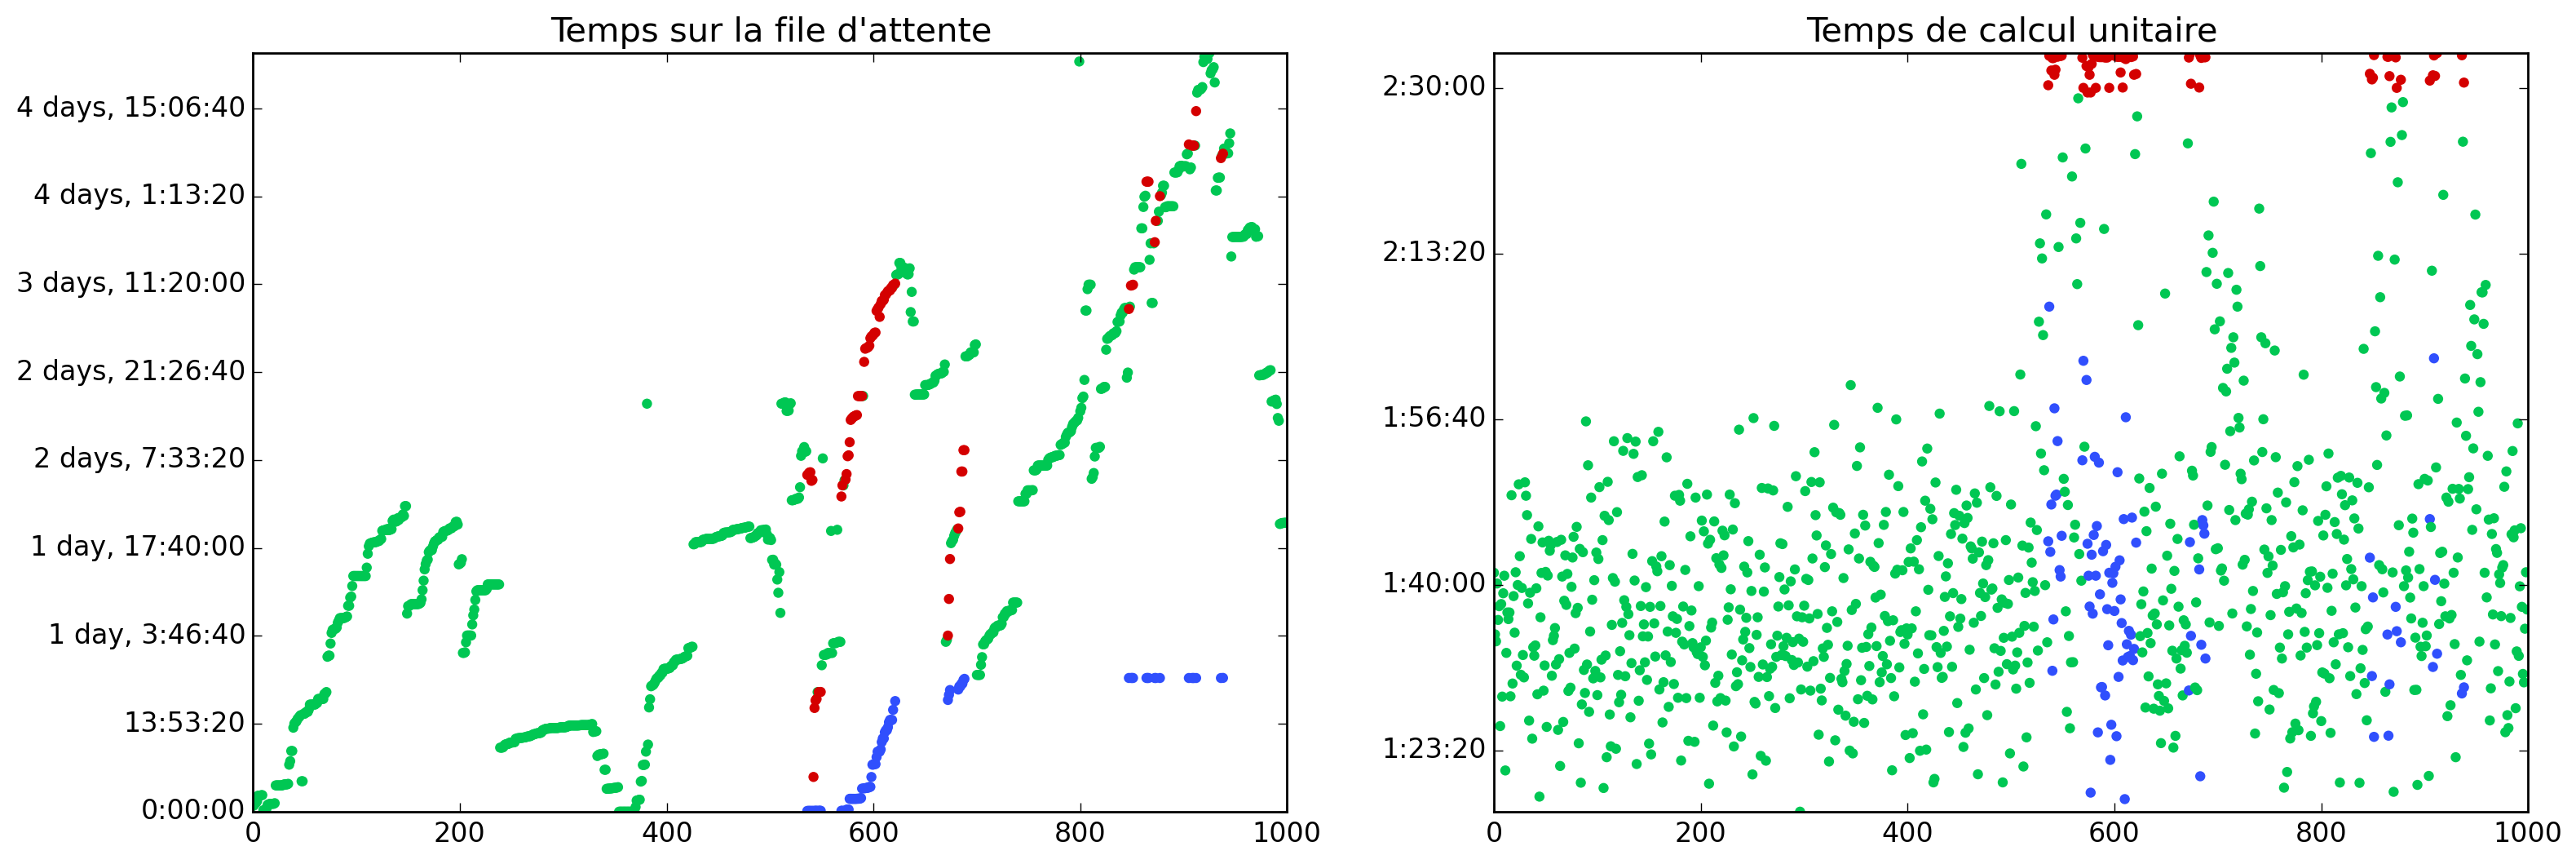
\includegraphics[width=0.9\textwidth]{./figure/Temps_DOE_Sobol_1000-white.png}
\end{frame}


\begin{frame}[fragile]
\frametitle{Parse output parameters 1/2}
\begin{itemize}
\item Common practice among scientific code is to create output files with
  the results of the simulation.
\item The output should then be parsed in order to get the output
  parameters of interest.
\item If it is a \texttt{.csv} file
\begin{itemize}
    \item \href{http://pandas.pydata.org/pandas-docs/stable/generated/pandas.read_csv.html}{pandas.read\_csv} is the fastest option, but it introduces pandas as a dependency.
    \item if speed is not an issue, try \href{http://doc.openturns.org/openturns-latest/sphinx/user_manual/_generated/openturns.coupling_tools.get_value.html}{ot.coupling\_tools.get\_value}, 
    \item or \href{http://docs.scipy.org/doc/numpy-1.10.0/reference/generated/numpy.loadtxt.html}{numpy.loadttxt}.
\end{itemize}
\end{itemize}
\end{frame}

\begin{frame}[fragile]
\frametitle{Parse output parameters 2/2}
\begin{itemize}
\item For \texttt{.xml} files, \href{https://docs.python.org/2/library/xml.dom.minidom.html}{minidom} package from the python standard library does the trick.
\item If the external code returns the output parameters of
  interest to STDOUT, set \texttt{get\_stdout=True} when calling
  \texttt{ot.coupling\_tools.execute(...)}.  (or use \href{https://docs.python.org/2/library/subprocess.html#subprocess.check_output}{subprocess.check\_output})
\item For standard binary formats, there are python interfaces to \href{https://github.com/Unidata/netcdf4-python}{netcdf}
  and \href{http://www.h5py.org/}{HDF5}.
\item Otherwise, be creative and pythonic !
\end{itemize}
\begin{Verbatim}[xleftmargin=10mm]
def _parse_output(self):
    # Retrieve output (see also )
    xmldoc = minidom.parse('outputs.xml')
    itemlist = xmldoc.getElementsByTagName('outputs')
    Y = float(itemlist[0].attributes['Y1'].value)

    return [Y]
\end{Verbatim}
\end{frame}


\section{In use tools}
\label{sec-4}
\begin{frame}[fragile]
\frametitle{Managing data backups}
\begin{itemize}
\item 2 useful functions:  \href{http://openturns.github.io/otwrapy/master/_generated/otwrapy.dump_array.html}{otwrapy.dump\_array} and  \href{http://openturns.github.io/otwrapy/master/_generated/otwrapy.load_array.html}{otwrapy.load\_array}
\begin{itemize}
	\item Fast solution.
	\item Data can be compressed (\texttt{gzip} library). If the extension is \texttt{`pklz`}, compression is automatic.
	\item Tips: Convert your \texttt{ot.Sample} to a \texttt{np.array} before, it is lighter !
\end{itemize}

\item Dump and compress
\end{itemize}
\begin{Verbatim}[xleftmargin=10mm]
import otwrapy as otw
otw.dump_array(np.array(X), 'InputSample.pklz', compress=True)
\end{Verbatim}

\begin{itemize}
\item ... and load
\end{itemize}
\begin{Verbatim}[xleftmargin=10mm]
import otwrapy as otw
import openturns as ot
X = otw.load_array('InputSample.pklz')
X = ot.Sample(X)
\end{Verbatim}
\end{frame}

\begin{frame}[fragile]
\frametitle{Catch exceptions when your code fails}
\begin{itemize}
\item In order to catch exceptions: \href{http://openturns.github.io/otwrapy/master/_generated/otwrapy.Debug.html}{otwrapy.Debug()} !
\begin{itemize}
\item Avoids crashes, raises exceptions and saves logs.
\item Useful when the wrapper is not used on an interactive environment (IPython, Jupyter notebook).
\end{itemize}

\end{itemize}
\begin{Verbatim}[xleftmargin=10mm]
import otwrapy as otw
class Wrapper(ot.OpenTURNSPythonFunction):
    @otw.Debug('wrapper.log')
    def _exec(self, X):
        #Do stuff
        return Y
\end{Verbatim}
\end{frame}

\begin{frame}[fragile]
\frametitle{Creating a CLI for your wrapper}
\begin{itemize}
\item Command Line Interface (CLI): to run your wrapper in detached mode, e.g., through submission scripts on HPC clusters.
\item The \href{https://docs.python.org/3/library/argparse.html}{argparse} library might be useful to link the python code with the external code.
\item Take a look at the \href{https://github.com/openturns/otwrapy/tree/master/otwrapy/examples/beam}{beam wrapper}  for an example of a CLI interface
\end{itemize}
\begin{Verbatim}[xleftmargin=10mm]
if __name__ == '__main__':
    import argparse
    parser = argparse.ArgumentParser(description="Python wrapper example.")
    parser.add_argument('-X', nargs=3, metavar=('X1', 'X2', 'X3'),
        help='Vector on which the model will be evaluated')
    args = parser.parse_args()

    model = Wrapper(3, 1)
    X = ot.Point([float(x) for x in args.X])
    Y = model(X)
    dump_array(X, 'InputSample.pkl')
    dump_array(Y, 'OutputSample.pkl')
\end{Verbatim}
\begin{itemize}
\item You can then execute your code from the command line :
\end{itemize}
\begin{Verbatim}[xleftmargin=10mm]
python wrapper.py –X 170 3 0.05
\end{Verbatim}
\end{frame}

\section{Parallelization}
\label{sec-7}
\begin{frame}[fragile]
\frametitle{Parallelizing the wrapper}
\begin{itemize}
\item Uncertainty studies imply independant and repetitive tasks: very simple to parallelize.
\item One function: \href{http://openturns.github.io/otwrapy/master/_generated/otwrapy.Parallelizer.html}{otwrapy.Parallelizer()} !!
\end{itemize}
\begin{Verbatim}[xleftmargin=10mm]
import otwrapy as otw
from otwrapy.examples.beam import Wrapper
parallelized_beam_wrapper = otw.Parallelizer(Wrapper())
\end{Verbatim}
\end{frame}


\begin{frame}
\frametitle{Distributing calls on clusters or the cloud}
\begin{itemize}
\item otw.Parallelizer is no longer the way to go\ldots{}
\item You can manage to make an heterogeneous office cluster with \href{http://ipyparallel.readthedocs.io/en/latest/}{IPyparallel} or \href{http://dispy.sourceforge.net/}{dispy}
\item For clusters and the cloud, rely on a good CLI interface of your
  wrapper and distribute your calls through submission scripts or
  cloud APIs (e.g., \href{https://www.simulagora.com/}{Simulagora} or \href{https://www.dominodatalab.com/}{Domino})
\end{itemize}
\end{frame}


\section{Conclusion}
\label{sec-8}
\begin{frame}
\frametitle{Conclusion}
\begin{itemize}
\item Main steps:
\begin{itemize}
	\item build your simulation code, and define inputs and outputs;
	\item identify ways to communicate inputs and outputs;
	\item make a wrapper to drive your simulation with python (>> otwrappy makes it easier);
	\item distribute your computations (>> otwrappy makes it easier).
\end{itemize}

\item By creating a CLI of your wrapper, you can easily distribute your calls on a cluster or on cloud platforms.
\item It is important to protect your wrapper with otw.Debug() so that you can have a traceback of raised Exceptions.

\item \href{http://openturns.github.io/otwrapy/master/index.html}{otwrapy} is here for you ! Use it to avoid code boilerplate or as a simple cookbook.
\end{itemize}
\end{frame}


\begin{frame}
\frametitle{Thank you for your attention}

\begin{center}

\includegraphics[width=0.15\textwidth]{./figure/LogoPhiHaut-white.png}
\vfill
Gaëtan Blondet
\vfill
\href{mailto:blondet@phimeca.com}{blondet@phimeca.com}
\vfill
Github : \href{http://openturns.github.io/otwrapy/master/index.html}{otwrapy}
\end{center}
\end{frame}

\end{document}
